\documentclass[a4paper, landscape, twocolumn, 11pt]{article}
\usepackage{layout}
\usepackage{lipsum}
\setlength\intextsep{0pt}
\begin{document}
\section*{FPGA - Field Programmable Gate Array}

\begin{wrapfigure}{r}{0.6\linewidth}
    \centering
    \vspace{20pt}
    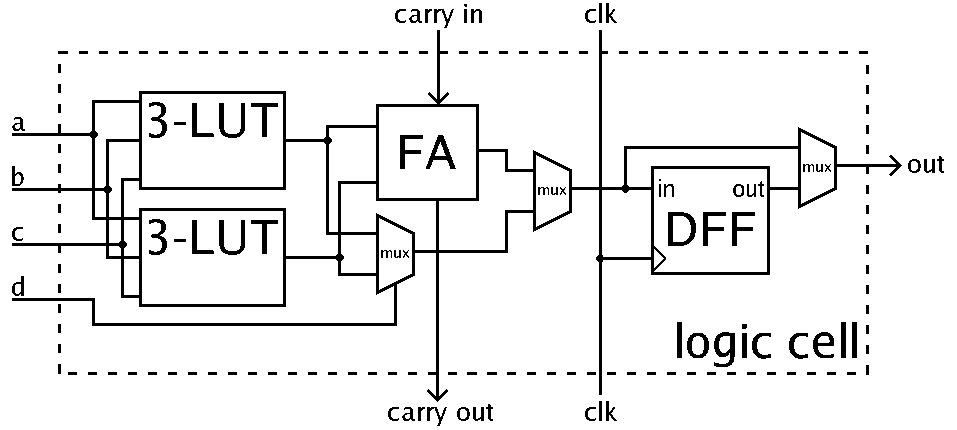
\includegraphics[width=1.0\linewidth]{fig/FPGA_cell_example.png}
    \caption{Illustration of a logic cell with three-input LUTs, full-adder and 
        D-type flipflop (picture from \protect\cite{wiki:fpga})}
    \label{fig:logic_cell}
    \vspace{20pt}
    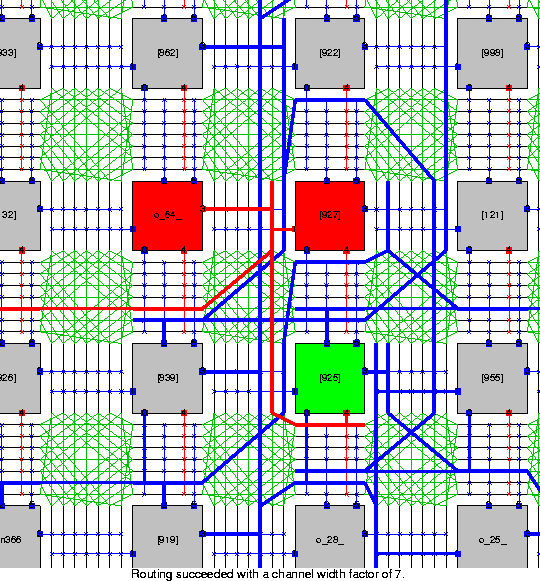
\includegraphics[width=1.0\linewidth, trim=0 10 0 0, clip=true]{fig/rr_graph.png}
    \caption{Illustration of logic cells connected through routing channels 
        (picture from \protect\cite{betz:fpga_arch})}
    \label{fig:logic_cell}
    \vspace{-1000pt}
\end{wrapfigure}
\subsection*{Overview}
\begin{itemize}
    \item Invented 1985 by Xilinx
    \begin{itemize}
        \item XC2064
        \item 64 CLBs
    \end{itemize}
    \item 2015:
    \begin{itemize}
        \item Xilinx Virtex UltraScale+
        \item 3.3 billion CLBs
    \end{itemize}
\end{itemize}

\subsection*{Internal structure}
\begin{itemize}
    \item Logic cells (CLB 
        \footnote{\textbf{C}onfigurable \textbf{L}ogic \textbf{B}lock})
    \begin{itemize}
        \item Lookup table (LUT)
        \item Full-adder
        \item D-type flipflop
    \end{itemize}
    \item Routing channels to connect CLBs
    \item Block RAM\footnote{\textbf{R}andom \textbf{A}ccess \textbf{M}emory}
    \item DSP\footnote{\textbf{D}igital \textbf{S}ignal \textbf{P}rocessing} 
        blocks
    \item Hard blocks
    \begin{itemize}
        \item Multi-gigabit-transceivers
        \item Processor cores
        \item Ethernet MACs
        \item Memory controllers
    \end{itemize}
\end{itemize}

\subsection*{Area of application}
\begin{itemize}
    \item Aerospace and defense
    \item Automotive
    \item Broadcast
    \item Medical electronics
    \item Wired and wireless communication
\end{itemize}

\subsection*{Applications}
\begin{itemize}
    \item Digital signal processing
    \item ASIC prototyping
    \item Motor control
    \item Image processing
    \item Data mining
    \item cell phone base station
\end{itemize}

\newpage
\subsection*{Comparison to CPU\footnote{
    \textbf{C}entral \textbf{P}rocessing \textbf{U}nit} solution}
\noindent
\begin{minipage}[t]{0.485\linewidth}
    \subsubsection*{Advantages}
    \begin{itemize}
        \item Faster for parallel processible tasks
        \item Number of I/O pins
    \end{itemize}
\end{minipage}
\begin{minipage}[t]{0.02\linewidth}
    ~
\end{minipage}
\begin{minipage}[t]{0.485\linewidth}
    \subsubsection*{Disadvantages}
    \begin{itemize}
        \item High power consumption
        \item High unit costs
        \item Sensitive to radiation
    \end{itemize}
\end{minipage}

\subsection*{Comparison to ASIC\footnote{
    \textbf{A}pplication \textbf{S}pecific 
    \textbf{I}ntegrated \textbf{C}ircuit} solution}
\noindent
\begin{minipage}{0.485\linewidth}
    \subsubsection*{Advantages}
    \begin{itemize}
        \item Field reprogrammability
        \item Low initial costs
        \item Faster time-to-market
    \end{itemize}
\end{minipage}
\begin{minipage}{0.02\linewidth}
    ~
\end{minipage}
\begin{minipage}{0.485\linewidth}
    \subsubsection*{Disadvantages}
    \begin{itemize}
        \item High power consumption
        \item High unit costs
        \item Bigger form-factor
        \item Sensitive to radiation
    \end{itemize}
\end{minipage}

\begin{figure}[h!]
    \vspace{11pt}
    \centering
    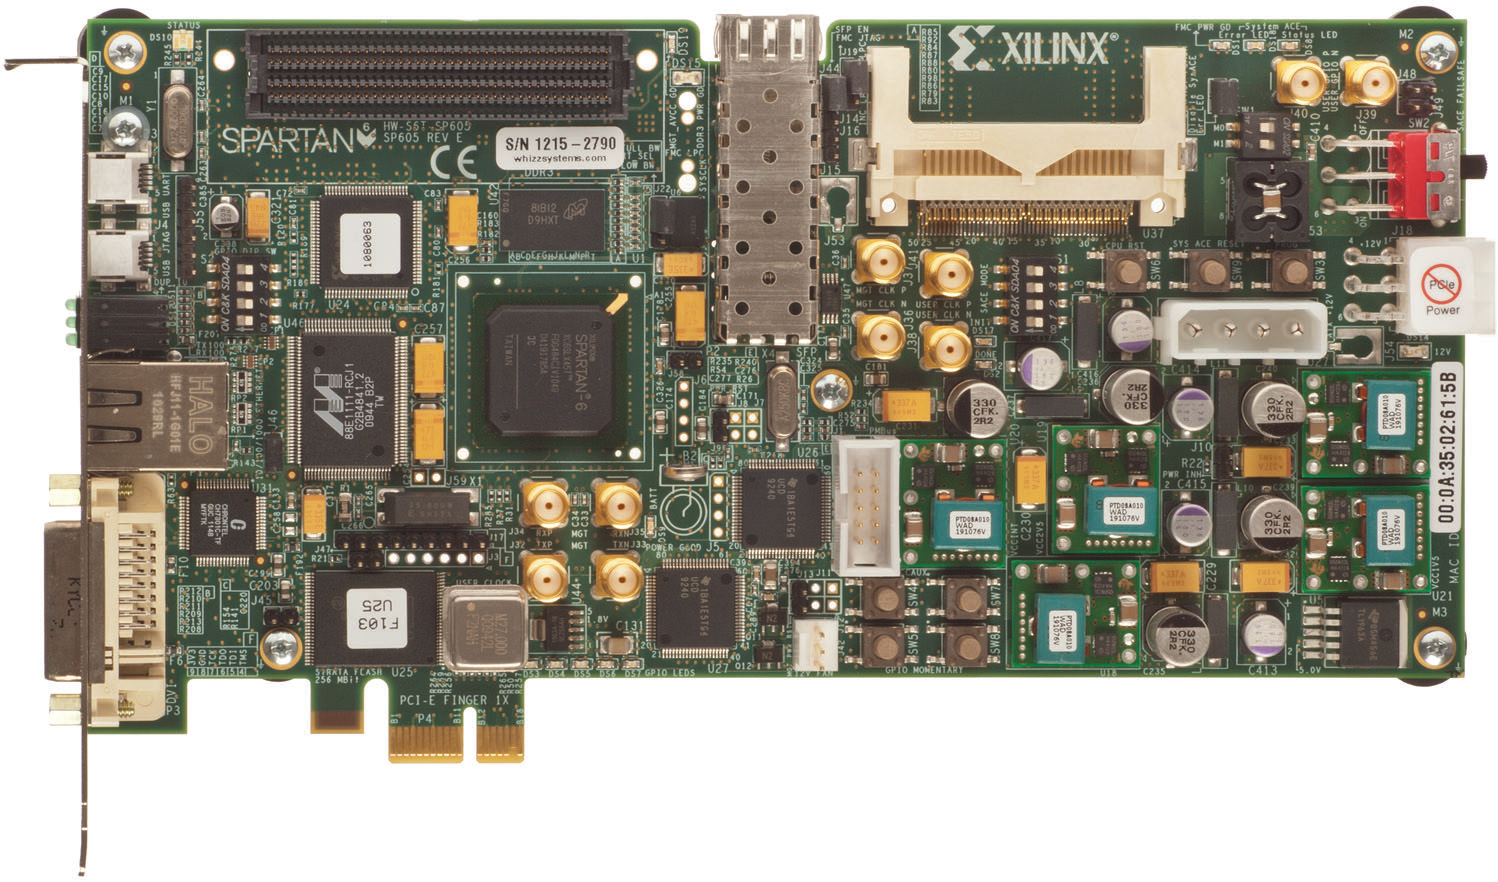
\includegraphics[width=0.8\linewidth]{fig/sp605.png}
    \caption{Development board with Xilinx Spartan 6 FPGA (picture from 
        \url{http://www.xilinx.com/support/documentation/boards_and_kits/ug526.pdf})}
    \label{fig:devboard}
\end{figure}

\nocite{*}
\bibliography{factsheet}
\end{document}
